% MBS Thesis Proposal - TU Faculty of Management
% Topic: Accounting Fundamentals and Post-Disclosure Share Prices: Evidence from Selected Nepalese Commercial Banks
% Format source: Master's Degree Dissertation Guidelines 2019, Office of the Dean FOM TU
%   -> proposal = flat sections i-vii, 8-12 pages, APA 6th, TNR 12pt, 1.5 spacing
% Engine: xelatex + bibtex (uses the actual Times New Roman system font)
\documentclass[12pt,a4paper,oneside]{article}

\usepackage{fontspec}
\setmainfont{Times New Roman}
\usepackage{newtxmath}

% Guideline p.20-21: top/bottom/right 2.54 cm, LEFT 3.18 cm
\usepackage[top=2.54cm,bottom=2.54cm,right=2.54cm,left=3.18cm]{geometry}

\usepackage{setspace}
\onehalfspacing                 % guideline: 1.5 spacing
\setlength{\parindent}{0pt}    % paragraphs start flush left

\usepackage{titlesec}
\usepackage{titletoc}
\usepackage{fancyhdr}
\usepackage{graphicx}
\usepackage{booktabs}
\usepackage{array}
\usepackage{longtable}
\usepackage{needspace}
\usepackage{amsmath}
\usepackage{tikz}
\usetikzlibrary{shapes,arrows,positioning}

% Guideline: APA sixth edition (explicit in Ch. I and Appendix C)
\usepackage[natbibapa]{apacite}
\bibliographystyle{apacite}
\usepackage{caption}
\captionsetup{font={normalsize,bf},justification=justified,singlelinecheck=false}
\usepackage{hyperref}
\hypersetup{colorlinks=true,linkcolor=black,citecolor=black,urlcolor=black}

% TU-strict front-matter headings (guideline p.9)
\renewcommand{\contentsname}{Table of Contents}
\renewcommand{\listtablename}{List of Tables}
\renewcommand{\listfigurename}{List of Figures}

% Match TOC entry typography to the corresponding body headings.
\titlecontents{section}
  [1.1em]
  {\addvspace{12pt}\normalfont\large\bfseries}
  {\contentslabel[\thecontentslabel.]{1.1em}}
  {\hspace*{-1.1em}}
  {\titlerule*[0.5pc]{.}\contentspage}
\titlecontents{subsection}
  [2.5em]
  {\addvspace{5pt}\normalfont\normalsize}
  {\contentslabel{1.4em}}
  {}
  {\titlerule*[0.5pc]{.}\contentspage}

% Section and subsection labels follow the active LaTeX counters.
\renewcommand{\thesection}{\arabic{section}}
\titleformat{\section}{\normalfont\bfseries\large}{\thesection.}{0.5em}{}
\titleformat{name=\section,numberless}{\normalfont\bfseries\fontsize{16pt}{20pt}\selectfont\centering}{}{0pt}{}
\titlespacing*{\section}{0pt}{18pt}{8pt}
\titlespacing*{name=\section,numberless}{0pt}{18pt}{14pt}

\renewcommand{\thesubsection}{\thesection.\arabic{subsection}}
\titleformat{\subsection}{\normalfont\bfseries\normalsize}{\thesubsection}{0.5em}{}
\titlespacing*{\subsection}{0pt}{12pt}{4pt}
\titleformat{\subsubsection}{\normalfont\bfseries}{}{0pt}{}
\titlespacing*{\subsubsection}{0pt}{10pt}{4pt}

% The literature review uses starred subheadings; methodology uses numbered
% subsections, which LaTeX adds to the TOC automatically.
\setcounter{secnumdepth}{2}
\setcounter{tocdepth}{2}

% Page numbering: front matter uses Roman numerals; body uses Arabic numerals.
% This proposal places both in the bottom centre.
\pagestyle{fancy}
\fancyhf{}
\fancyfoot[C]{\thepage}
\renewcommand{\headrulewidth}{0pt}
\setlength{\headheight}{15pt}

\begin{document}

% --- Title page: counted, but unnumbered (guideline p.21).
% NOTE: \thispagestyle{empty} lives INSIDE front/titlepage.tex -- it must run
% before the titlepage environment issues its page break, or it blanks p.2.
\begin{titlepage}
\thispagestyle{empty}
\singlespacing
\setlength{\parskip}{0pt}
\begin{center}

{\fontsize{18}{22}\selectfont\bfseries VALUE RELEVANCE OF ACCOUNTING INFORMATION BEFORE AND AFTER THE BANKING CONSOLIDATION WAVE: EVIDENCE FROM NEPALESE COMMERCIAL BANKS\par}

\vspace{2.2cm}

{\fontsize{16}{20}\selectfont\bfseries A Dissertation Proposal\par}

\vspace{2.0cm}

{\fontsize{13}{16}\selectfont A Dissertation Proposal Submitted to\par}
\vspace{0.25cm}
{\fontsize{13}{16}\selectfont\bfseries Office of the Dean\par}
{\fontsize{13}{16}\selectfont\bfseries Faculty of Management\par}
{\fontsize{13}{16}\selectfont\bfseries Tribhuvan University\par}

\vspace{1.5cm}

{\fontsize{12}{16}\selectfont \textit{In partial fulfillment of the requirements for the Degree of\\Master of Business Studies (MBS)}\par}

\vspace{1.8cm}

{\fontsize{13}{16}\selectfont Submitted by\par}
\vspace{0.25cm}
{\fontsize{12}{16}\selectfont\bfseries Asmita Subedi\par}
{\fontsize{12}{16}\selectfont Triveni International College\par}
{\fontsize{12}{16}\selectfont Exam Roll No: 67514/24\par}
{\fontsize{12}{16}\selectfont T.U. Regd. No: 7-2-48-1060-2018\par}

\vfill

{\fontsize{12}{15}\selectfont Pokhara, Nepal\par}
{\fontsize{12}{15}\selectfont October, 2026\par}

\end{center}
\end{titlepage}



% --- Front matter (FOM 2019: Table of contents; p.20: single spacing)
% Title page = i (counted, unnumbered). Front matter = ii bottom centre.
% NOTE: LOT/LOF removed -- proposal contains zero tables and one figure;
% a blank LOT page and one-line LOF page read as padding. TOC only.
\pagenumbering{roman}
\setcounter{page}{2}
\begingroup
\singlespacing
\tableofcontents
\clearpage
\endgroup

% --- Main body sections 1-7 ---
% Body restarts at Arabic 1; page numbers remain bottom-centred.
\pagenumbering{arabic}
\setcounter{page}{1}
\fancyhf{}
\fancyfoot[C]{\thepage}
\renewcommand{\headrulewidth}{0pt}
\setlength{\headheight}{15pt}

% --- Proposal structure 1-7 ---
\section{Background of the study}

The stock market plays an important role in economic development by promoting
capital formation and fostering economic growth. Trading of securities facilitates
savers and users of capital by fund pooling, risk sharing, and transferring wealth
\citep{mosley2008}.

In Nepal, the organized stock market began with the conversion of the Securities
Exchange Centre into Nepal Stock Exchange (NEPSE) Limited in 1993, with floor
trading commencing in 1994. NEPSE remains the sole stock exchange in the country
and has grown substantially in both market capitalization and the number of listed
securities.

Returns from equity investments vary with firm performance and stock price
movements driven by technical, fundamental and market-sentiment factors
\citep{bhattarai2014}. In the Nepalese banking sector, earnings per share (EPS),
price-earnings (P/E) ratio, dividend per share (DPS), book value per share (BVPS)
and return on assets (ROA) are established firm-specific determinants of share
prices \citep{bhattarai2014,pradhan2016,sharma2011}.

The Nepalese banking sector has undergone substantial restructuring through the
merger and acquisition wave of 2013--2020 and the consolidation of early 2023:
Global IME Bank absorbed Bank of Kathmandu, Kumari Bank absorbed Nepal Credit
and Commerce Bank, Nepal Investment Bank merged with Mega Bank to form Nepal
Investment Mega Bank, and Himalayan Bank acquired Civil Bank
\citep{adhikari2023}. Across the broader financial sector, 239 banking and
financial institutions entered merger processes and 177 ceased to exist in their
own names, with the commercial-bank count falling from 32 in 2014 to 20 by
mid-2023. Sector-wide market price per share fell by roughly 46\% in the
periods following the mergers while earnings and dividend per share were
statistically unchanged \citep{adhikari2023,adhikari2023cbr}. The existing
share-price literature is based on pre-consolidation data and samples that no
longer reflect the current structure of the industry. The conflicting findings
on ROA and BVPS across recent studies further underscore the need for a
comprehensive empirical examination of the fundamental determinants of share
prices in the post-consolidation banking sector.

\section{Problem statement}

Several commercial-bank mergers began joint operation in early 2023, changing
the ownership and reporting boundaries of the affected institutions
\citep{nrb2023list}. The present study does not treat this consolidation as a
causal intervention. Its problem is narrower: reported findings on the
association of accounting fundamentals, particularly ROA and BVPS, with bank
share prices differ across studies, samples, and periods.

For example, Chhetri (2023) reports a positive ROA coefficient, whereas
Chaudhari (2025) reports a negative coefficient and Gyawali (2022) reports a
positive but statistically insignificant ROA coefficient. Joshi et al. (2023)
report a positive BVPS association, whereas Pant et al. (2024) report a
negative, statistically insignificant BVPS coefficient. These estimates are
not directly comparable without considering their different samples, periods,
variable definitions, and model specifications. Further, studies by Pant et al.
(2024), Chaudhari (2025), and Timalsina (2026) include observations through FY
2023/24, so the case for this proposal cannot be that all prior evidence
predates the major 2023 consolidation. The proposed study is a bounded
extension: it applies a stated post-disclosure price-date rule to a target of
five purposively selected bank series through FY 2081/82. It describes
associations in those series; it does not identify a merger effect or a change
in coefficients across periods.

The study addresses the following questions:
{\renewcommand{\theenumi}{\roman{enumi}}
\begin{enumerate}
  \item What levels and fiscal-year patterns do EPS, DPS, BVPS, ROA, and post-disclosure market price per share show in the sampled bank series?
  \item How is each of EPS, DPS, BVPS, and ROA associated with post-disclosure market price per share?
  \item How are EPS, DPS, BVPS, and ROA jointly associated with post-disclosure market price per share?
\end{enumerate}
}

\section{Objectives of the study}

The primary objective of this study is to describe and estimate the
associations between selected accounting fundamentals and post-disclosure
market price per share ($\mathit{MPS}^{post}$) for five purposively selected
Nepalese commercial-bank series over FY 2076/77--2081/82. The analysis spans
the early-2023 consolidation period but does not estimate a merger effect or
test for a structural break. The specific objectives are:
\begin{enumerate}
  \item To describe the levels and fiscal-year patterns of EPS, DPS, BVPS, ROA, and $\mathit{MPS}^{post}$ in the sampled bank series.
  \item To estimate the bivariate associations between each accounting fundamental and $\mathit{MPS}^{post}$.
  \item To estimate the joint and conditional associations of EPS, DPS, BVPS, and ROA with $\mathit{MPS}^{post}$ using the stated regression model.
\end{enumerate}

\section{Hypothesis}

Based on accounting valuation arguments and the mixed empirical evidence
reviewed below, the study states the following expected positive associations.
The hypotheses describe expected coefficient signs; two-tailed tests are used
in the analysis, so statistical significance alone will not be treated as
confirmation of the expected direction:
\begin{itemize}
  \item $H_1$: There is a significant positive relationship between earnings per
    share (EPS) and post-disclosure market price per share ($\mathit{MPS}^{post}$).
  \item $H_2$: There is a significant positive relationship between dividend per
    share (DPS) and post-disclosure market price per share ($\mathit{MPS}^{post}$).
  \item $H_3$: There is a significant positive relationship between book value
    per share (BVPS) and post-disclosure market price per share ($\mathit{MPS}^{post}$).
  \item $H_4$: There is a significant positive relationship between return on
    assets (ROA) and post-disclosure market price per share ($\mathit{MPS}^{post}$).
\end{itemize}

\section{Rationale of the study}

The study provides a bounded description of how selected accounting measures
are associated with share prices observed after audited financial statements
are disclosed for up to five purposively selected bank series. The six-year window
includes the early-2023 consolidation, but the design does not estimate a
merger effect, establish causal determinants, or support generalization to all
commercial banks. Its practical value depends on whether the disclosure dates,
market prices, and accounting measures can be constructed consistently for
every sampled bank-year. If the data are complete and comparable, the results
may offer investors, bank managers, regulators, and future researchers a
transparent description of these sampled series. The small purposive sample,
merger-related changes in reporting boundaries, and exploratory regression
inference limit the strength and reach of any conclusions.

\section{Brief review of the literature}

\subsection*{Theoretical review}

Equity valuation provides a basis for examining reported accounting measures in
relation to share prices. Miller and Modigliani's dividend-irrelevance result
holds under restrictive assumptions, including fixed investment policy and
frictionless capital markets; under those assumptions, changing the payout
does not by itself change firm value \citep{miller1961}. This result is a
benchmark rather than a direct prediction that a higher observed dividend per
share must be associated with a higher market price in Nepal.

Signaling theory offers a conditional reason why accounting disclosures and
dividend decisions may be associated with price. Ross (1977) models financial
structure choices as signals when managers have information unavailable to
investors. Bhattacharya (1979) develops a separate model in which dividends can
signal managers' expectations of future profitability under specified
information and signaling-cost assumptions. These theories do not establish
that every dividend increase signals stronger performance; they motivate
examining DPS alongside the other reported measures \citep{ross1977,
bhattacharya1979}.

Ohlson's valuation model relates market value to current and future earnings,
book values, dividends, and other information, with the clean-surplus relation
providing an accounting foundation \citep{ohlson1995}. In the present study,
EPS represents earnings on a per-share basis, BVPS represents book equity on a
per-share basis, DPS records the reported distribution for the fiscal year,
and ROA represents reported asset profitability. EPS and ROA share an earnings
numerator, while DPS and BVPS are also related to earnings and retained
earnings. The regressors are therefore not assumed to be statistically
independent; their overlap is one reason to assess multicollinearity and to
interpret conditional coefficients cautiously.

Several Nepalese studies include the price-earnings ratio (P/E) alongside
market price per share (MPS) as an explanatory variable \citep{bhattarai2014,
chhetri2023}. Because P/E is calculated as MPS divided by EPS, it is
mathematically coupled to this study's dependent variable. This proposal
therefore excludes P/E from its regression. This is a specification choice for
the present model, not a claim that all prior studies using P/E are invalid.

\subsection*{Empirical review}

International studies provide context but are not direct evidence for the
Nepalese banking sample. Research on NSE 100 firms in India and listed banks in
Jordan examines combinations of earnings, book value, dividends, and valuation
multiples, with findings depending on the market, sample, and specification
\citep{malhotra2013,almumani2014}. Earlier Nepalese bank studies by Bhattarai
(2014) and Pradhan and Dahal (2016) also report associations between accounting
fundamentals and share prices, but their observation periods end before the
early-2023 merger wave \citep{bhattarai2014,pradhan2016}.

More recent Nepalese studies do not yield a uniform result for all variables.
Gyawali (2022), using ten banks over 2017--2021, reports a positive but
statistically insignificant ROA coefficient. Chhetri (2023) studies 13 banks
over 2012--2022 using pooled cross-sectional analysis; the paper reports
positive, statistically significant results for BVPS and ROA and includes P/E
in a model with MPS as the outcome. Joshi et al. (2023) report a positive BVPS
association in their commercial-bank sample. These estimates differ in sample,
period, variable construction, and model specification, so they should not be
treated as estimates of one common effect \citep{gyawali2022,chhetri2023,
joshi2023}.

Studies with periods extending through FY 2023/24 provide evidence from the
post-consolidation period. Pant et al. (2024), using seven purposively selected
banks, report a negative, statistically insignificant BVPS coefficient.
Chaudhari (2025), using ten banks, reports a significantly negative ROA
coefficient. The abstract of Timalsina (2026), which covers 13 banks through
FY 2023/24, reports no statistically significant ROA association. These
studies show that post-consolidation-period evidence exists, but their results
remain mixed across samples, periods, and specifications \citep{pant2024,
chaudhari2025,timalsina2026}.

Merger evidence must also be distinguished by period and outcome. Adhikari,
Kavanagh, and Hampson (2023) compare financial ratios before and after mergers
for seven commercial banks involved in transactions from 2013 to 2020. Their
reported 46.01\% fall in mean MPS is specific to that sample and period; it is
not an estimate for the early-2023 mergers \citep{adhikari2023}. Other work
examines post-merger financial performance or governance rather than the
disclosure-timed share-price outcome used here \citep{adhikari2023cbr,
bhattarai2024,dongol2024}.

\subsection*{Research gap}

The reviewed literature includes studies with observations through FY
2023/24, so this proposal does not claim that post-consolidation evidence is
absent. Instead, it asks what bivariate and conditional associations are
observed in a target of five purposively selected bank series over FY 2076/77--2081/82
when MPS is measured using one explicit rule: the NEPSE closing price on the
first trading day after the corresponding audited annual financial statements
are publicly disclosed through NEPSE. This rule makes the proposed price
observation reproducible; it is not, by itself, evidence that the design is
novel. The study does not test merger effects or resolve conflicting findings
across different studies.

The analysis estimates bivariate associations and a joint pooled-OLS
specification for EPS, DPS, BVPS, and ROA with post-disclosure MPS. It excludes
P/E because that ratio is constructed from MPS and EPS. Findings will be
interpreted for the sampled bank series only, with the small sample and
changes in reporting boundaries around mergers treated as limitations.

\section{Research methodology}

\msub{1.1.1 Research design}
This study uses a quantitative, descriptive and correlational design with
secondary data \citep{pant2016}. The descriptive analysis summarizes the
levels and fiscal-year patterns of EPS, DPS, BVPS, ROA, and
$\mathit{MPS}^{post}$. Pearson correlations describe pairwise associations,
and pooled ordinary least squares (OLS) estimates the joint conditional
associations specified in Eq.~\ref{eq:main}. The intended sample is five bank
series observed in each of six fiscal years, FY 2076/77--2081/82, for a target
of 30 bank-year observations, subject to verification of the underlying
reports and trading records. Completeness is not assumed before data
collection. Any unavailable or unverifiable observation will be identified
and reported, and will not be imputed silently. If one or more observations
cannot be established, the realized sample and implications for estimation
will be reported. The design specifies six annual observations for each bank
series, but four series cross a merger boundary: pre-merger observations refer
to the acquiring institution and later observations refer to the consolidated
institution. These series are not unchanged legal entities throughout the
period. The OLS analysis is exploratory; its conventional significance tests
do not account for possible within-series dependence and will not be treated
as confirmatory evidence or as causal effects.

\msub{1.1.2 Population and sampling procedure}
The target population for the post-consolidation sample frame is the 20
commercial banks listed by Nepal Rastra Bank as of mid-October 2023
\citep{nrb2023list}. From this population, a
sample of 5 commercial banks is selected using a purposive (judgmental) sampling
technique. The selection criteria require: (i) representation of the prominent
commercial bank mergers that defined the early 2023 consolidation wave, (ii)
inclusion of an unmerged reference bank (NMB Bank) for descriptive context,
and (iii) continuous availability of audited annual financial statements,
NEPSE trading records, and accounting measures by their relevant observation
dates across the entire study period. Because the
sample is non-probabilistic and comprises 5 institutions, the empirical findings
are interpreted specifically for the sampled banks and serve as an indicative
benchmark rather than an automatic generalization across all 20 commercial
banks.

The sampled commercial banks, identified by their current legal corporate names,
are:
\begin{enumerate}
  \item Global IME Bank Limited (absorbed Bank of Kathmandu, joint operation commenced 9 January 2023, swap ratio 1:1) \citep{gbime2022agm,nrb2023list}
  \item Himalayan Bank Limited (acquired Civil Bank, joint operation commenced 24 February 2023, swap ratio 100:80.28) \citep{hbl2023report}
  \item Kumari Bank Limited (absorbed Nepal Credit and Commerce Bank, joint operation commenced 1 January 2023, swap ratio 1:1) \citep{kumari2022sgm,nrb2023list}
  \item Nepal Investment Mega Bank Limited (merger of Nepal Investment Bank and Mega Bank, joint operation commenced 11 January 2023, swap ratio 100:90) \citep{nimb2023report}
  \item NMB Bank Limited (maintained independent operations without merger during the period) \citep{nrb2023list}
\end{enumerate}
For each merged bank series, pre-merger observations represent the acquiring
institution and post-merger observations represent the consolidated
institution. The fiscal year in which a merger began joint operation is a
transition year: the audited statement's reporting boundary will be recorded
for each bank-year, and that observation will be flagged rather than described
as a clean pre-merger or post-merger year. The merger changes the scale and
composition of the series; regression coefficients are not interpreted as
causal estimates of merger effects. The study covers FY 2076/77--2081/82,
spanning years before, during, and after the early-2023 mergers, targeting 30
observations (5 bank series $\times$ 6 fiscal years), subject to the stated
data-availability criteria. The single unmerged series
provides descriptive context only; the model does not estimate a merger-versus-
non-merger comparison.

\msub{1.1.3 Nature and sources of data collection}
This study relies entirely on secondary financial and market data. Bank
financial statements provide the accounting measures; NEPSE trading records
provide market prices. NRB, SEBON, and Ministry of Finance publications
provide regulatory and sector context and are used for cross-checking where
they report the same observation. Sources for each bank-year are recorded in
the data file. The principal sources are:
\begin{itemize}
  \item Audited annual reports and published financial statements of the sampled commercial banks.
  \item \textit{Banking and Financial Statistics} and supervision reports published by Nepal Rastra Bank (NRB).
  \item Trading records, official share price bulletins, and annual publications of the Nepal Stock Exchange (NEPSE) and the Securities Board of Nepal (SEBON).
  \item \textit{Economic Survey} published by the Ministry of Finance (MoF), Government of Nepal.
\end{itemize}
Extracted figures are checked against the originating report and, where an
independent source reports the same measure, cross-checked before processing.
Differences are recorded and resolved using the originating audited report for
accounting measures and the NEPSE record for trading prices.

\msub{1.1.4 Research framework and definition of variables}
The research framework illustrating the functional relationship between the
explanatory accounting fundamentals and the dependent variable is depicted in
Figure~\ref{fig:framework}. Post-disclosure market price per share
($\mathit{MPS}^{post}$) serves as the dependent variable, while earnings per share
(EPS), dividend per share (DPS), book value per share (BVPS), and return on assets
(ROA) are the explanatory variables.

\begin{figure}[h]
\centering
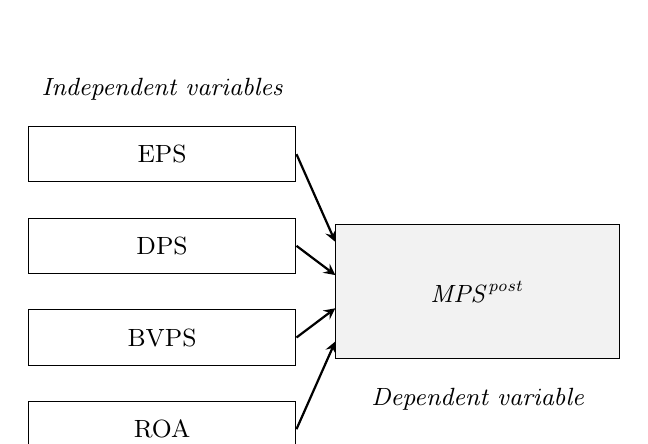
\begin{tikzpicture}[node distance=0.45cm,
  ind/.style={rectangle, draw, minimum width=3.4cm, minimum height=0.7cm, text centered, font=\small},
  dep/.style={rectangle, draw, minimum width=3.6cm, minimum height=1.7cm, text centered, font=\small, fill=gray!10},
  arrow/.style={thick,->,>=stealth}]
  \node[ind] (eps)  {EPS};
  \node[ind, below=of eps] (dps)  {DPS};
  \node[ind, below=of dps] (bvps) {BVPS};
  \node[ind, below=of bvps] (roa) {ROA};
  \path (dps) -- (bvps) coordinate[midway] (mid);
  \node[dep, right=2.2cm of mid] (mps) {$\mathit{MPS}^{\mathit{post}}$};
  \draw[arrow] (eps.east)  -- ([yshift=18pt]mps.west);
  \draw[arrow] (dps.east)  -- ([yshift=6pt]mps.west);
  \draw[arrow] (bvps.east) -- ([yshift=-6pt]mps.west);
  \draw[arrow] (roa.east)  -- ([yshift=-18pt]mps.west);
  \node[above=0.2cm of eps, font=\small\itshape] {Independent variables};
  \node[below=0.25cm of mps, font=\small\itshape] {Dependent variable};
\end{tikzpicture}
\caption{Research framework (Source: adapted from Pradhan and Dahal, 2016)}
\label{fig:framework}
\end{figure}

Post-disclosure market price per share ($\mathit{MPS}^{\mathit{post}}$),
measured in Nepalese rupees (NPR), is the closing price on the first NEPSE
trading day after public disclosure of the corresponding audited annual
financial statements through NEPSE. The same rule is applied across all
sampled banks and fiscal years. The statement disclosure date, trading date,
and source records are logged for each bank-year. If a bonus issue, rights
issue, split, or other
share-capital action affects the quoted price between fiscal year-end and the
measurement date, the event and any price adjustment are documented using
NEPSE or issuer notices; adjusted and unadjusted prices are not mixed. Earnings
per share (EPS), in NPR per share, is profit attributable to ordinary equity
holders divided by the weighted-average ordinary shares outstanding, as
reported in or calculated from the audited statements. Dividend per share
(DPS), in NPR per share, is the amount reported for the corresponding fiscal
year; the data record identifies whether it is recommended, approved, or
distributed and records its public disclosure date. A DPS value that was not
publicly disclosed by the MPS observation date is recorded as unavailable and
is not used in the regression for that bank-year. Book value per share (BVPS), in
NPR per share, is the reported figure in the audited annual report. Return on
assets (ROA), in percent, is net profit after tax divided by year-end total
assets and multiplied by 100. For every bank-year, the data record identifies
the audited-report numerator and denominator and preserves any reported ROA
formula. ROA is recalculated from audited figures using the common definition
where both components are available. If a required figure cannot be
established, ROA is recorded as unavailable; a value using a different
denominator convention is not pooled with this measure.

\needspace{6\baselineskip}
\msub{1.1.5 Methods of analysis}
To examine the empirical relationships and evaluate the hypotheses formulated in
this study, both descriptive and inferential econometric techniques are applied.

\textbf{Model Specification:}
To examine the joint and conditional associations of all four accounting
fundamentals with post-disclosure market price per share, the following multiple
linear regression model is specified:
\begin{equation}
\mathit{MPS}^{post}_{it} = \beta_0 + \beta_1 \mathit{EPS}_{it} + \beta_2 \mathit{DPS}_{it} + \beta_3 \mathit{BVPS}_{it} + \beta_4 \mathit{ROA}_{it} + \varepsilon_{it}
\label{eq:main}
\end{equation}
where $\mathit{MPS}^{post}_{it}$ represents the closing market price observed
at the pre-specified post-disclosure trading date for bank $i$ in fiscal year
$t$. $\mathit{EPS}_{it}$, $\mathit{DPS}_{it}$, $\mathit{BVPS}_{it}$, and
$\mathit{ROA}_{it}$ denote earnings per share, dividend per share, book value
per share, and return on assets, respectively. The parameter $\beta_0$ represents
the intercept, $\beta_1$ through $\beta_4$ represent regression slope coefficients
capturing the estimated conditional association between each regressor and
$\mathit{MPS}^{post}$ holding the other included variables constant, and
$\varepsilon_{it}$ is the stochastic disturbance term.

\textbf{Statistical Tools and Estimation Procedure:}
The empirical analysis follows this protocol. Data suitability and model
assumptions are assessed before coefficient tests are interpreted:
\begin{enumerate}
  \item \textbf{Descriptive Statistics:} The mean, standard deviation, minimum,
    and maximum of all variables are computed to examine distributional
    properties across the panel.
  \item \textbf{Correlation Analysis:} Pearson correlations measure bivariate
    associations between each fundamental and $\mathit{MPS}^{post}$ and screen
    for collinearity among regressors.
  \item \textbf{Multiple Regression Analysis:} Eq.~\ref{eq:main} is
    estimated by pooled OLS as an exploratory baseline. The coefficient of
    determination ($R^2$) and adjusted $R^2$ describe in-sample fit. Individual
    coefficients are assessed with two-tailed $t$-tests at the 5\% level
    ($\alpha=0.05$), and joint model significance is assessed with an $F$-test
    at the 5\% level. Since the intended 30 observations repeat five bank series and
    four series cross merger boundaries, these conventional model-based tests
    are interpreted cautiously; they do not establish causal effects or
    sector-wide relationships.
  \item \textbf{Diagnostic Tests:} Model assumptions are examined before interpreting results.
    Multicollinearity is evaluated with variance inflation factors (VIF) and tolerance statistics alongside the correlation matrix.
    Residual diagnostics include checks for heteroskedasticity (White or
    Breusch-Pagan test), influential observations (Cook's distance), and
    residual distribution (Q-Q plot). The correlation matrix, VIF, and
    tolerance are reviewed for multicollinearity. Residual patterns are also
    inspected by bank series and fiscal year because repeated observations may
    be dependent. With only five bank series, bank-clustered standard errors
    would rely on very few clusters; conventional cluster-based tests can
    over-reject with small cluster counts \citep{cameron2008clusters}. They are
    therefore not treated as an automatic remedy. The small sample,
    transition-year reporting boundaries, and limits of conventional OLS
    inference are stated with the results. If diagnostics indicate serious
    violations, coefficient tests will not be presented as suitable for
    confirmatory interpretation.
\end{enumerate}

Data organization, coding, descriptive statistics, correlations, pooled OLS,
and the specified diagnostic checks are conducted using Microsoft Excel and
the Statistical Package for the Social Sciences (SPSS).


% --- References (apacite prints its own heading) ---
% References always start on a fresh page. Listed in the TOC (thesis-style).
\clearpage
\phantomsection
\addcontentsline{toc}{section}{References}
\begingroup
\singlespacing
\interlinepenalty=10000 % Keep each bibliography entry together across page breaks.
\bibliography{references}
\endgroup

\end{document}
